% Couverture Thèse TPT Latex v2
% Fabrice Linot 04/12/11 

\documentclass[11pt,a4paper]{book}
\usepackage[left=1.3cm,top=0cm,right=1.3cm,bottom=1.2cm]{geometry}
\usepackage{graphicx}
\usepackage{eso-pic}
\usepackage{array}
\usepackage[english]{babel}
\usepackage[utf8x]{inputenc}
\usepackage[T1]{fontenc}
\usepackage{textcomp}
\usepackage{hyperref}
\usepackage{natbib}
\usepackage{helvet}	% or \usepackage{lmodern}
\renewcommand\textnumero{n$^{\textsf{{\tiny O}}}$}
\renewcommand{\familydefault}{\sfdefault}

\hypersetup{
    colorlinks,
    citecolor=red,
    filecolor=black,
    linkcolor=blue,
    urlcolor=blue
}

\usepackage{ifpdf}
\newcommand\BackgroundPic{
\ifpdf
	\includegraphics[height=\paperheight,width=\paperwidth]{cover_bg.pdf}
\else
	\includegraphics[height=\paperheight,width=\paperwidth]{cover_bg.pdf}
\fi}

\pagestyle{empty}

\begin{document}
\AddToShipoutPicture*{\BackgroundPic}
~

\begin{flushright}

\includegraphics[scale=0.45]{logo_TPT.pdf}

{\small {2015-ENST-00xx~~~~}}
\end{flushright}



%\vspace{0.cm}
\begin{center}
%


\includegraphics[scale=0.65]{logo_edite.pdf} \\
{\small {EDITE - ED 130}}


%
\vspace{.5cm}
%
%
%
%{\Large École doctorale \textnumero XX: texte}\\		% version une ligne
%{\Large École doctorale \textnumero XX:\\ texte}\\		% version deux lignes (changer les espaces en conséquence
%
%
%
\vspace{1.0cm}
%
%
%
{\LARGE {\bf Doctorat ParisTech}}\\
\vspace{1.1cm}
{\LARGE {\bf T H È S E}}\\
\vspace{0.5cm}
{\normalsize {\bf pour obtenir le grade de docteur délivré par}}\\
%
%
%
\vspace{.9cm}
%
%
%
%
{\LARGE {\bf TELECOM ParisTech}}\\
\vspace{0.6cm}
{\Large {\bf Spécialité Xxxx }}\\
%
%
%
\vspace{.8cm}
%
%
%
{\normalsize {\it présentée et soutenue publiquement par}}\\
\vspace{0.7cm}
{\Large {\bf Mainak JAS}}\\
\vspace{0.24cm}
{\normalsize le jour mois année}\\
%
%
%
\vfill
%
%
%
\textcolor[RGB]{191,18,56}{
\noindent
{\LARGE {\bf Advances in automating analysis of\\[.6cm]neural time series data}}\\
}
%
%
%
\vfill~\vfill
%
%
%
{\normalsize
\begin{tabular}{c}
Directeur de thèse:					{\bf Alexandre GRAMFORT}\\
Co-encadrement de la thèse:		{\bf Prénom NOM}
\end{tabular}
}
\end{center}
%
%
%
\vfill
%
%
%
\flushleft
\begin{minipage}{.9\textwidth}	% ou .91\textwidth si vous n'avez pas assez de place
{\bf Jury}\\
% Mme/M. Prénom NOM, Titre, Unité de recherche, Ecole 
{\bf Mme/M. Prénom NOM}, {\small Titre, Unité de recherche, Ecole}
	\hfill Fonction\\
{\bf Mme/M. Prénom NOM}, {\small Titre, Unité de recherche, Ecole}
	\hfill Fonction\\
{\bf Mme/M. Prénom NOM}, {\small Titre, Unité de recherche, Ecole}
	\hfill Fonction\\
{\bf Mme/M. Prénom NOM}, {\small Titre, Unité de recherche, Ecole}
	\hfill Fonction\\
{\bf Mme/M. Prénom NOM}, {\small Titre, Unité de recherche, Ecole}
	\hfill Fonction\\
{\bf Mme/M. Prénom NOM}, {\small Titre, Unité de recherche, Ecole}
	\hfill Fonction\\
{\bf Mme/M. Prénom NOM}, {\small Titre, Unité de recherche, Ecole}
	\hfill Fonction\\
{\bf Mme/M. Prénom NOM}, {\small Titre, Unité de recherche, Ecole}
	\hfill Fonction\\

\end{minipage}\\
%
%
%
\vspace{-.3cm}
%
%
%
{\centering
{\bf TELECOM ParisTech}\\
{\small école de l'Institut Mines-Télécom - membre de ParisTech}\\
{\tiny 46 rue Barrault 75013 Paris - (+33) 1 45 81 77 77 - www.telecom-paristech.fr}}
%
%
%
%
\newpage
\tableofcontents
\listoffigures
\listoftables
\chapter{Introduction}

Understanding the human brain is one of the most significant challenges of the 21st century. The brain is responsible

\section{Modern brain imaging}

\begin{figure}[htb]
\begin{center}
   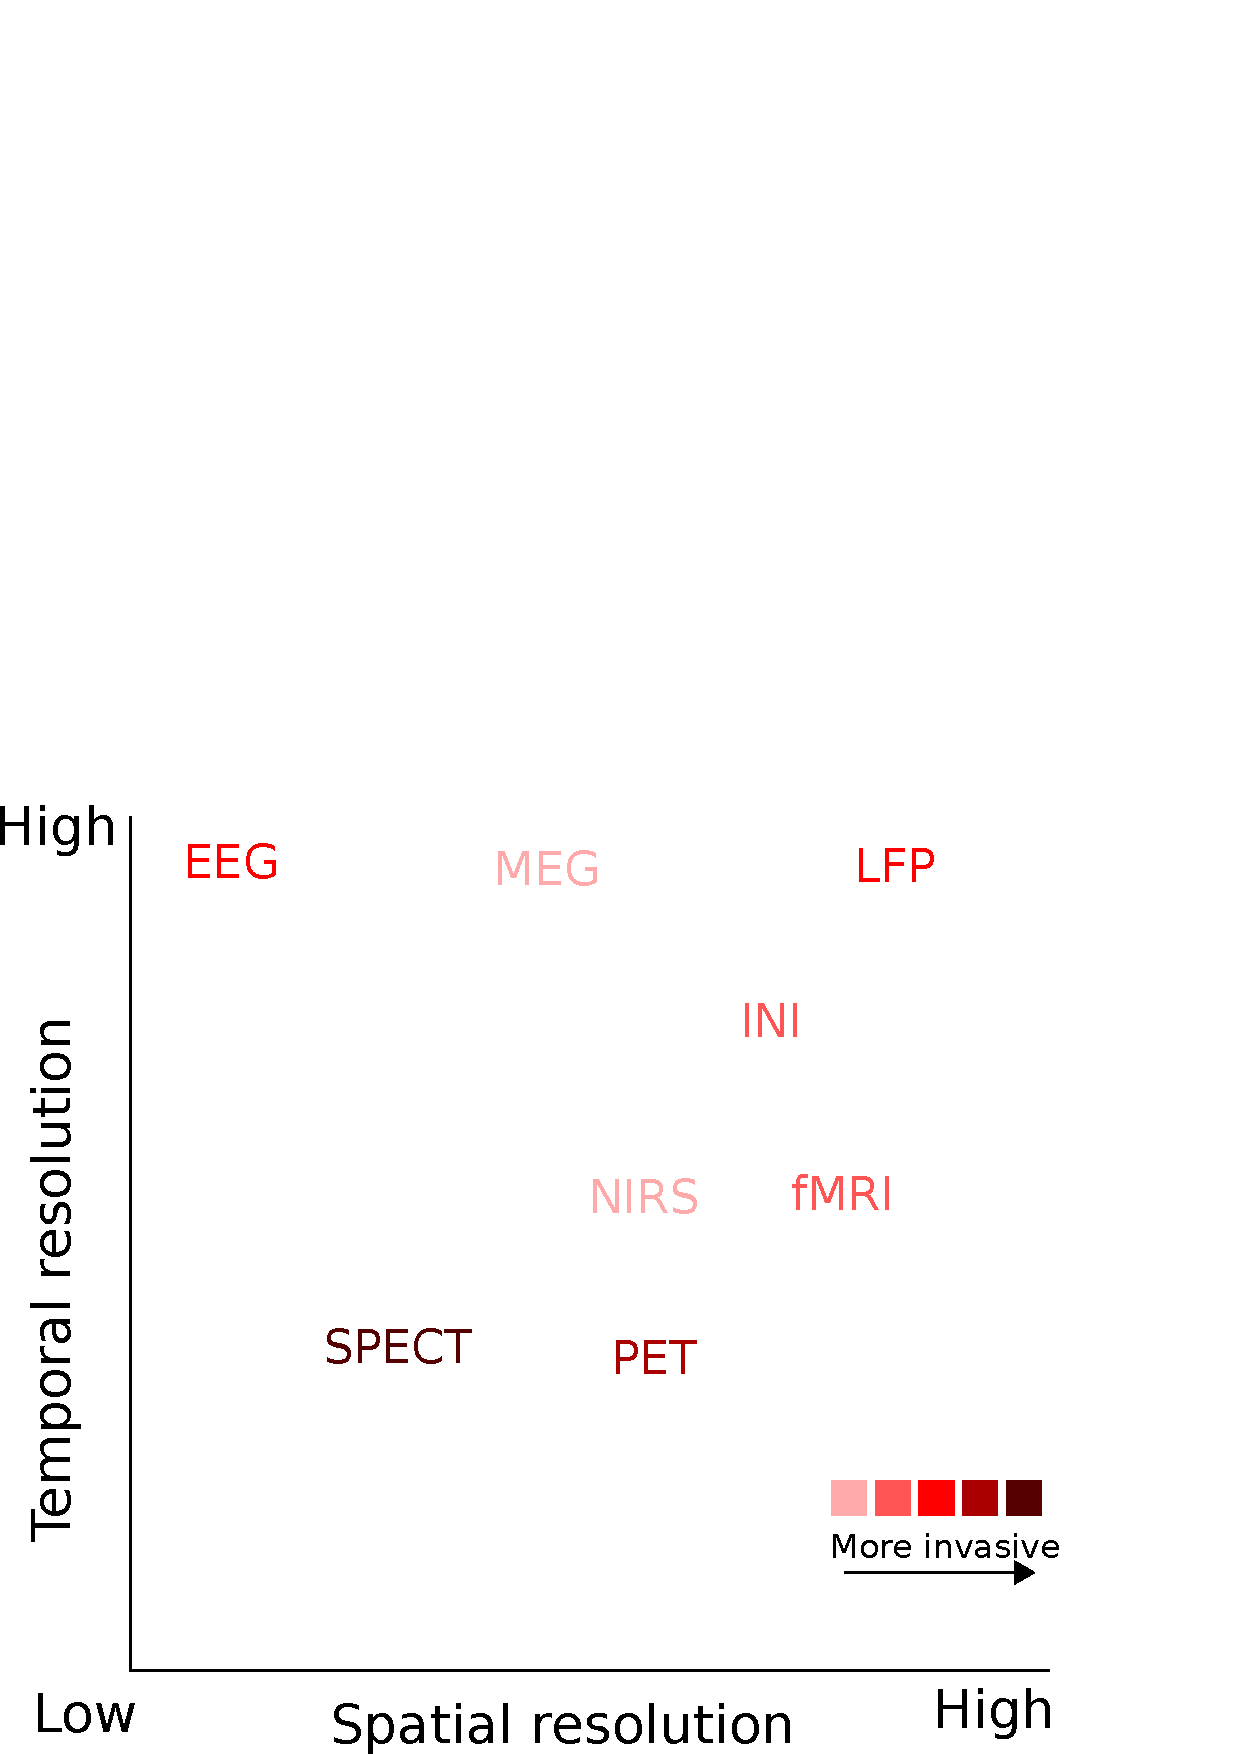
\includegraphics[width=0.4\linewidth]{figures/neuroimaging_methods.pdf}
\end{center}
   \caption{Various neuroimaging methods differ in terms of the information they measure. MEG=magnetoencephalography, EEG=electroencephalography, NIRS=near-infrared spectroscopy, PET=positron emission tomography, SPECT=single photon emission tomography, and INI=Inverse imaging, a method to speed up acquisition of fMRI images.}
   \label{fig:neuroimaging_methods}
\end{figure}

\section{The reproducibility crisis}

Even though thousands of papers are published every year about different aspects of the brain, our understanding of this complex organ has not scaled in proportion. A large part of the reason has been attributed to what is known as the replication crisis~\citep{ioannidis2005most, simmons2011false, button2013power}. Replication is closely related to the concept of reproducibility which refers to the idea that an experiment produces the same result when performed again under the same conditions. Replication is a stronger condition as it requires similar results or identical conclusion even if there are some minor variations in the experimental procedures. Progress in science rests on the reproducibility of experiments. In many fields, however, a large fraction of experiments cannot be reproduced. In psychology, for instance, it was estimated that over half of the papers were not reproducible~\citep{open2015estimating}, and even those reproduced tended to have a weaker effect size compared to the original study. 

This has led the field to look introspectively

preregistration, publishing negative results
 This is due to a number of reasons such as confirmation bias, pressure to publish and absence of incentives to publish negative results, ``p-hacking''~\citep{simmons2011false}. However, brain imaging has its own set of issues which can be linked to replication crisis:

% vul2009puzzlingly
% yendiki2014spurious

\begin{itemize}[noitemsep,nolistsep]
\item Multiple comparison
\item Differences in software
\item Complex pipelines~\citep{Carp2012289}
\item \emph{Power failure}, or the tendency to conduct studies using sample sizes thereby increasing the likelihood of a false discovery just by chance.
\item Head movements~\citep{yendiki2014spurious}
\item Lack of data
\end{itemize}

Lack of data and power failure are related

list the reasons for reproducibility crisis and how it's unique for neuroimaging as opposed to behavioral sciences

reverse inference

dead salmon~\citep{bennett2009neural}

\section{Data sharing}
The history of data sharing can be traced back to Newton and his theory of gravitation~\citep{pointofview2013}. Before Newton had developed his theory, another English astronomer, John Flamsteed had been appointed by the king to observe the stars and produce accurate charts for navigation in the seas. Over a period of 40 years, Flamsteed created a detailed catalogue that tripled the number of entries in the previously used sky atlas. When the great comet of 1680 appeared in the sky twice in close succession, Flamsteed used his data to postulate that it was not two comets but in fact the same comet which first went towards the sun and then turned away from it. Newton initially opposed this theory, but later changed his mind as he gained access to Flamsteed's unpublished catalogue. The comet had indeed turned out to be an important benchmark for Newton's theory of gravitation.

It is hard to imagine in this day and age that a theory as fundamental as the laws of gravitation could have been data driven. Today, data sharing is fundamental to reproducible science, but it also forms the cornerstone for learning better models and benchmarking new algorithms. If one follows the breakthroughs in the field of machine learning, for instance, it is predicated on the availability of data. It is an almost undisputed fact that the recent resurgence of deep learning owes in part at least, to the release of Imagenet~\citep{deng2009imagenet}. The same is true for Q learning in Atari games~\citep{watkins1992q, bellemare2013arcade}, natural language processing for language translation [ref], speech recognition [ref], and even the mixture of experts model~\citep{jacobs1991adaptive} for IBM Watson~\citep{ferrucci2010building}. If such datasets were available in neuroscience, we would be able to tease apart even subtle effects that were not possible before with smaller sample sizes.

Of course, neuroscientists are beginning to realize the importance of sharing data. In recent times, neural data has started being shared through international consortiums~\citep{van2013wu, ollier2005uk} and data repositories~\citep{poldrack2013toward, gorgolewski2015neurovault}. While in the case of Newton, he gained access to the catalogue without permission, today it is possible to publish dataset papers in targeted journals so as to assign the credit where it is due.
Data sharing is beneficial not just from the perspective of replication but also from an economic perspective. Rather than collect new data for every new hypothesis, researchers can now reuse existing data for answering their hypotheses.

\subsection{Brain Imaging Data Structure}

While data sharing in neuroscience is on the rise, the amount of data reuse is still limited. For instance, since the release of the Human Connectome Project (HCP) [ref -- meg one] data in 2013 [check], there have been only one or two documented cases of reusing the MEG data. Even in these cases, the effort has mostly been to reproduce rather than test new hypotheses. This brings us to a crucial point: dataset sharing is not a panacea as the tools, skills and resources to process such large datasets is currently missing. Perhaps the most important roadblock is standardization of metadata. 

Neuroimaging experiments are often complicated involving different paradigms (auditory, visual, somatosensory \emph{etc.}), different acquisition parameters (sampling frequency, number of sensors and their location, measurement device \emph{etc.}), and [subject's gender, age etc]. As if this weren't complicated enough, often intermediate results from the data are sometimes shared as well owing to the long preprocessing time. The data itself could be stored in 10--20 different file formats depending on the device used for acquisition. Therefore, it is almost a guaranteed fact that certain parameters will be missing or differently recorded when comparing across measurement sites.

A graduate student or postdoc who has newly started analyzing the data will be unable to make any progress unless all these different parameters are known beforehand. Combining different datasets, a first step towards making larger datasets, is almost out of question. To appreciate the importance of standardization, let us consider as a simpler example of the toy. Imagine, instead of the clocks that we know today, we had clocks that were nonstandard as in Figure [].

clock image [ref to design of everyday things]

Even though, it is easy to infer the time, it disturbs us. The reason is that we are used to reading clocks where the 12 o' clock mark is fixed at the top and the direction of motion is \emph{clockwise}. Indeed,

If we are to ever hope for crowdsourcing neural data acquisition, the first step must be standardizing the data formats.

\section{Automation}
Back in 2014, Nature published a bold article~\citep{hayden2014automated} which described a vision for the future: ``solving the problem of bringing McDonald's-like efficiency to scientists''. This would in turn lead to cheaper, more efficient and reliable research. While it goes on to describe many biology labs which are automating experiments, the benefits of automation in the neuroimaging community are yet to be widely recognized. But what are the opportunities for automation in the context of neuroimaging? Let us list down some of them:
\begin{itemize}[noitemsep,nolistsep,nosep]
\item \textbf{Data organization:} Neuroimaging data can often run into many Terabytes with intermediate files at different stages of processing. Keeping track of this heterogeneous data manually can be a challenging process.
\item \textbf{Parameter tuning:} Most algorithms, although automated, require hyperparameters to be tuned. This could be the number of trials to perform in an experiment, the number of components to select in a \ac{PCA} decomposition, or the regularization parameter in inverse solvers.
\item \textbf{Annotation and labeling:} The challenge of neuroimaging data is that it is often unlabeled. As reliable annotations can be performed only by experts, crowdsourcing is often not a possibility. The alternative is to automatically label different types of signals.
\item \textbf{Reporting and quality control:} Automated Statistician . \ac{MNE} web report
\end{itemize}
Ultimately, this will lead to higher quality of 

Efficiency, it turns out, is not simply a matter of scale. Even for moderately sized experiments,

% automated statistician
%
% This subjectivity can lead to studies which are not reproducible unless every single detail was carefully documented. Even then, it does not rule out a potential confirmation bias: the tendency to favor processing steps which leads one to confirm the hypothesis being tested rather than reject it.

data revolution


data sharing, data standards, open source

\subsection{Janitor work}

One of the biggest roadblocks to large scale analysis is what is known as `janitor work': the effort required to standardize a dataset before it is actually usable. In the context of neuroimaging, this can involve organizing files at different stages of processing, manually inspecting the data, annotating segments which contain artifacts, and even removing outlier subjects from the analysis. Merely based on anecdotal reports, we can conclude that this can take up to a week of time even for a moderately sized study of 10--20 subjects.
%If at some point, the researcher realized that a certain parameter early in the pipeline needed to be changed, this would entail redoing all the subsequent steps in the pipeline, including the manual processing. 
In addition to the cost of human labor, one cannot ignore the subjectivity that these steps produces which can be problematic for reproducibility. As the number of datasets shared increases and neuroscientists are forced to confront statistically rigorous approaches to data analysis, the time is ripe to automate as many steps of the pipeline as possible.

\section{Representation learning}

\section{Contributions}
In this thesis, I attempt to synthesize the lessons learned from analysing public neuroimaging data with open source software. To this effect, I participated in an effort to create an MEG standard for the Brain Imaging Data Structure (BIDS). I wrote the validator which helped create the MEG-BIDS compatible example datasets. As a long time contributor to MNE [ref], I led an effort to reanalyze a simple dataset for a reproducible group study. At the same time, we realized that reproducibility cannot be attained unless all steps of analysis pipeline are automated. This led us to develop a fully automated algorithm for artifact rejection and repair [ref]. Finally, we develop algorithms to learn new undiscovered motifs automatically from neural time series data. 

\subsection*{Journal publications}
\bibentry{jas2017autoreject} \\ \\
\bibentry{jas2017mne} \\ \\
\bibentry{galan2017meg}

\subsection*{Conference publications}
\bibentry{jas2016automated} \\ \\
\bibentry{jas2017learning}


\addcontentsline{toc}{chapter}{Bibliography}
\bibliographystyle{abbrvnat}
\bibliography{refs}

\end{document}
